\section{Phase II Step 3: C3 Gaming-Resistance Analysis}
\label{sec:phase2_c3_gaming_resistance}

The third Month 3 criterion evaluates how easily each metric can be manipulated. This is important because
developer-reputation systems can create incentives to optimize the measured signal rather than the underlying
maintenance behavior. The C3 scoring therefore asks whether gaming is difficult, costly, detectable, and
controllable with the evidence already available in the centralized Phase I outputs.

\subsection{Scoring protocol and artifacts}
\label{sec:c3_protocol_artifacts}

C3 uses a fixed five-dimension rubric. Each dimension is scored on a 0--2 scale, where higher values mean
stronger resistance to manipulation. A metric can receive a good C3 score even if it is not perfect, provided
that likely manipulation is visible and can be controlled through cross-checks.

\begin{table}[H]
\centering
\scriptsize
\renewcommand{\arraystretch}{1.08}
\begin{tabularx}{\textwidth}{p{2.1cm}p{3.7cm}X}
\toprule
\textbf{Dimension} & \textbf{Name} & \textbf{Meaning} \\
\midrule
C3\_D1 & Manipulation difficulty & How difficult it is to artificially improve the metric. \\
C3\_D2 & Manipulation cost & How much real work or coordination manipulation requires. \\
C3\_D3 & Detectability from current evidence & Whether manipulation can be flagged from existing Phase I artifacts. \\
C3\_D4 & Cross-metric consistency & Whether the metric can be checked against other candidate signals. \\
C3\_D5 & Residual-risk control & Whether remaining gaming risk is acceptable after safeguards. \\
\bottomrule
\end{tabularx}
\caption{C3 gaming-resistance rubric. Each dimension is scored from 0 to 2, with higher scores meaning stronger resistance.}
\label{tab:c3_rubric}
\end{table}

\begin{table}[H]
\centering
\scriptsize
\renewcommand{\arraystretch}{1.08}
\begin{tabularx}{\textwidth}{p{5.1cm}rX}
\toprule
\textbf{Artifact} & \textbf{Rows} & \textbf{Role} \\
\midrule
\path{out/c3_gaming_rubric_all.csv} & 5 & Fixed C3 scoring dimensions and definitions. \\
\path{out/c3_gaming_attack_surface_all.csv} & 10 & Metric-specific attack vectors, evidence fields, and safeguards. \\
\path{out/c3_gaming_scores_all.csv} & 25 & Per-metric, per-dimension scores with written rationales. \\
\path{out/c3_gaming_summary_all.csv} & 5 & Metric-level total score, band, strongest dimensions, and weakest dimensions. \\
\path{logs/c3_gaming_resistance_20260508.log} & 1 & Execution log for the C3 scoring run. \\
\bottomrule
\end{tabularx}
\caption{Phase II C3 gaming-resistance artifacts. Paths are relative to the Phase II analysis directory.}
\label{tab:c3_artifacts}
\end{table}

\subsection{Attack-surface summary}
\label{sec:c3_attack_surface}

The attack-surface matrix records likely manipulations and the current detection boundary. M1 can be inflated by
adding low-value code or vendored/generated source. M2 can be inflated through unnecessary rewrites or formatting
changes. M3 can be manipulated by splitting work into many commits or by automation-heavy activity. M4 is harder
to manipulate because it depends on relative ownership over a window, but it can still be distorted by one large
dominant change or by unresolved identity-linkage issues. M5 is conceptually attractive, but because the current
evidence excludes issue and pull-request event streams, responsiveness gaming cannot be audited in this dataset.

\subsection{C3 results}
\label{sec:c3_results}

\begin{table}[H]
\centering
\scriptsize
\renewcommand{\arraystretch}{1.08}
\begin{tabularx}{\textwidth}{p{0.8cm}p{3.2cm}p{2.0cm}ccX}
\toprule
\textbf{ID} & \textbf{Metric} & \textbf{Status} & \textbf{Score} & \textbf{Band} & \textbf{Interpretation} \\
\midrule
M4 & Ownership/concentration & Implemented & 9/10 & High & Strongest gaming-resistance profile, but still needs identity and dominance caveats. \\
M2 & Churn & Implemented & 7/10 & Medium & Manipulable through unnecessary churn, but current evidence gives useful detection signals. \\
M3 & Activity cadence & Implemented & 6/10 & Medium & Commit splitting is easy, so cadence needs churn, active-day, and bot cross-checks. \\
M1 & Snapshot size & Implemented & 5/10 & Medium & Safe as context, weak as direct reputation evidence because size can be inflated. \\
M5 & Maintenance responsiveness & Design extension & 3/10 & Low & Current evidence cannot detect responsiveness gaming; exclude from baseline PoC decision. \\
\bottomrule
\end{tabularx}
\caption{C3 gaming-resistance summary for the candidate metrics.}
\label{tab:c3_gaming_summary}
\end{table}

\begin{figure}[H]
\centering
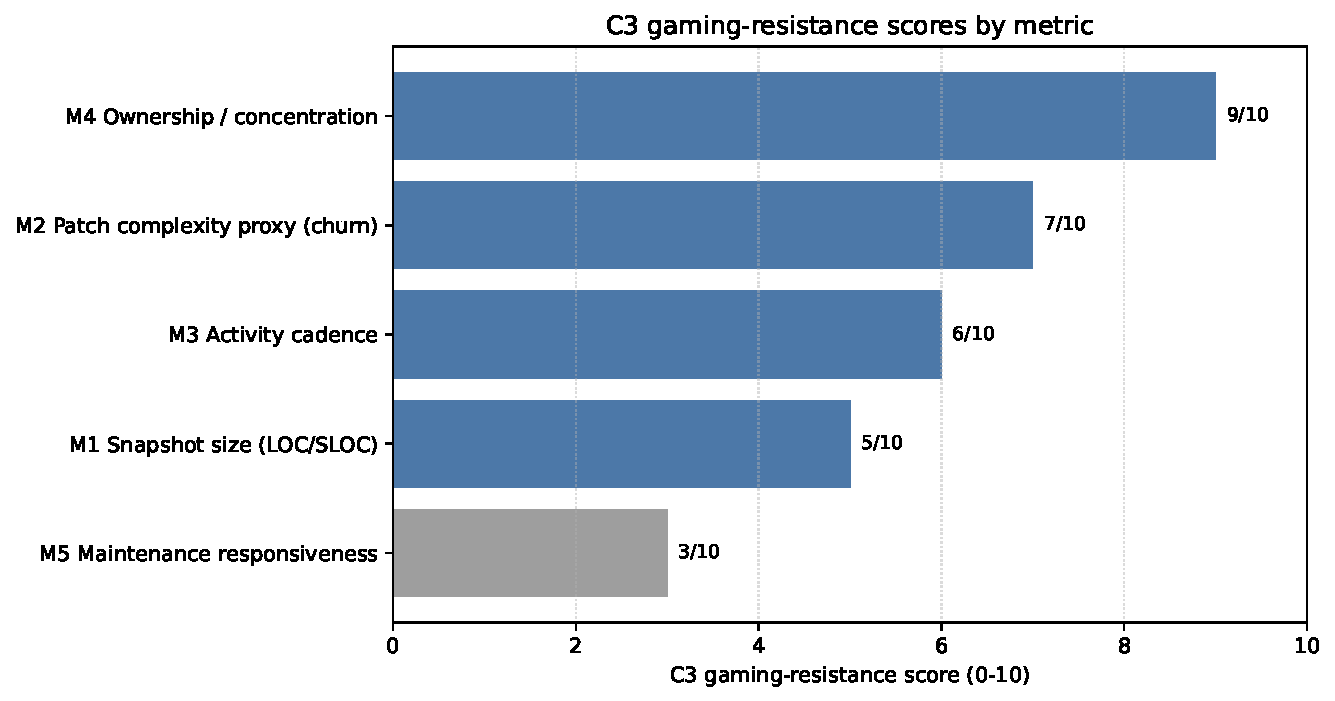
\includegraphics[width=0.90\textwidth]{figures/month3_c3/c3_gaming_resistance_scores.pdf}
\caption{C3 gaming-resistance scores on a 0--10 scale. Higher values indicate stronger resistance after safeguards.}
\label{fig:c3_gaming_scores}
\end{figure}

The C3 result changes the emphasis from C2. M3 was the most interpretable implemented metric, but it is easier
to manipulate through commit splitting. M4 is harder to explain, but it has the strongest resistance profile
because sustained ownership share is harder to fake than isolated commit counts or churn spikes. M2 remains useful
as effort evidence, but it should not be rewarded directly without checks against M3 cadence, M4 concentration,
LOC movement, and short-window flags. M1 remains appropriate as a context or normalization metric, not as a
standalone reputation score.

\subsection{C3 interpretation for the decision process}
\label{sec:c3_interpretation}

C3 does not select the PoC metric, but it introduces a strong warning against simple activity-based reputation:
\begin{itemize}[leftmargin=*]
  \item M1 should not be used directly for reputation because size is not maintainer quality.
  \item M2 is useful only when paired with safeguards against artificial churn.
  \item M3 is easy to explain but needs protection against commit splitting and bot-heavy activity.
  \item M4 is currently the strongest gaming-resistance candidate, provided identity handling and dominance spikes are documented.
  \item M5 remains excluded from the current empirical decision because the evidence needed to audit responsiveness is absent.
\end{itemize}

The next section evaluates C4 long-term suitability. That step checks whether each metric remains informative over
longer histories and whether it can be updated incrementally without recomputing the full project history.
